\section{Processi di supporto}


\subsection{Documentazione}

\subsubsection{Scopo}
Lo scopo di questa sezione è definire gli standard neccessari per la stesura di tutti i documenti del progetto.

\subsubsection{Ciclo di vita del documento}
Tutti i documenti prodotti dal team seguono la seguente ciclo di vita:
\begin{itemize}
    \item \textbf{Stesura}: il documento viene scritto utilizzando il metodo AGILE, adottando gli sprint di durata una settimana; 
    \item \textbf{Revisione}:a fine di ogni sprint i documenti vengono revisionati da una persona diversa dal redattore. Solo dopo la revisione
				le modifiche e i nuovi contenuti scritti possono essere integrati nel documento;
    \item \textbf{Verifica}:avviene in un periodo specificato nel piano di progetto, tale attività viene svolto da almeno una persona. Il documento
				è considerato verificato quando i Verificatori dichiarano che le modifiche neccessarie sono portate a termine;
    \item \textbf{Approvazione}:il Responsabile di Progetto dichiara che il documento è completo in ogni sua
					parte e pronto per essere rilasciato, marcandolo come approvato;
\end{itemize}
\begin{figure}[H]
    \centering
    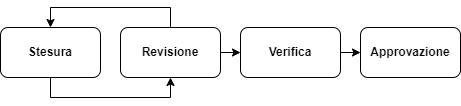
\includegraphics[scale=0.8]{img/ciclo_di_vita.png}
    \caption{Ciclo di vita dei documenti}
\end{figure}

\subsubsection{Struttura dei documenti}
Tutti i documenti ufficiali seguono una struttura ben definita cosi da mantenere l'omogeneità. Più precisamente ogni documento è formato da:
\begin{itemize}
    \item \textbf{Fontespizio};
    \item \textbf{Registro delle modifiche};
    \item \textbf{Indice};
    \item \textbf{Contenuto principale}.
\end{itemize}

\subsubsubsection{Fontespizio}
Rappresenta la pagina iniziale del documento ed è strutturato come segue:
\begin{itemize}
    \item \textbf{Logo dell'università}: logo dell'\textit{Università di Padova} posizionato in centro alto della pagina, seguito dalla nomenclatura "Università degli  Studi di Padova";
    \item \textbf{Logo del gruppo}: logo del gruppo, posizionato in centro, subito dopo la nomeclatura dell'università;
    \item \textbf{Nome del gruppo e del progetto}: il nome del gruppo e del capitolato scelto, seguito da un recapito email;
    \item \textbf{Nome del documento}: è il titolo del documento, definito in grassetto e posizionato al centro della pagina;
    \item \textbf{Tabella di descrizione}: è la tabella contenente le informazioni generali del documento.
\end{itemize}

\subsubsubsection{Registro delle modifiche}
I documenti che sono soggetti a modifiche periodiche sono dotati di un registro che ne memorizza lo storico. Il registro è fomato cosi:
\begin{itemize}
    \item \textbf{Versione}: indica la versione del documento dopo la modifica;
    \item \textbf{Descrizione}: descrive brevemente la modifica apportata;
    \item \textbf{Data}: indica la data in cui è stata modificata il documento.
\end{itemize}

\subsubsubsection{Indice}
Per agevolare la lettura, tutti i documenti sono dotati di un indice. Le sezioni sono rappresentati da un numero seguiti dal titolo della sezione, ogni sottosezione deve riportare il numero della sezione madre e poi il numero proprio. I numeri devono partire dall'1.

\subsubsubsection{Contenuto principale}
La pagina del contenuto è costituita da:
\begin{itemize}
    \item \textbf{Intestazione}: in alto a sinistra deve esserci il nome del gruppo \textit{Catch em All}, in altro a destra si trova il numero e nome della sezione in cui si trova;
    \item \textbf{Pie di pagina}: in basso sinistra si trova il nome del documento e la sua versione attuale, in basso a destra viene indicato il numero della pagina in cui si trova e il numero di pagine complessive del documento.
\end{itemize}

\subsubsection{Classificazione dei documenti}
Tutti i documenti prodotti sono divisi in uso interno e uso esterno:
\begin{itemize}
    \item \textbf{Uso interno}: sono documenti finalizzati a un uso interno al gruppo, tra cui \textit{Norme di progetto} e \textit{Verbali interni};
    \item \textbf{Uso esterno}: sono documenti di interesse a tutti gli stakeholder, tra cui \textit{Analisi dei requisiti}, \textit{Verbali esterni}, \textit{Piano di progetto}, (da completare).
\end{itemize}

\subsubsection{Norme tipografiche}

\subsubsubsection{Nome del file}
Di seguito viene descritto il formato dei nomi dei documenti:
\begin{itemize}
\item Iniziano tutti con la lettera minuscola;
\item Se il nome comprende più parole allora ognuna di esse è separata dal simbolo '\_';
\item Deve essere seguito da un indicazione della propria versione.
\end {itemize}
La sigla della versione deve essere così strutturata:
\begin{center}
    \large{\textbf{v.X.Y.Z}}
\end{center}
\begin{itemize}
\item \textbf{X} indicato da un numero che parte da 0, corrisponde al numero di approvazioni del documento da parte del responsabile;
\item \textbf{Y} indicato da un numero che parte da 0, corrisponde al numero di verifiche del documento da parte del verificatore, viene portato a 0 ad ogni incremento di \textbf{X};
\item \textbf{Z} indicato da un numero che parte da 0, corrisponde al numero di modifiche del documento da parte del redattore, viene portato a 0 ad ogni incremento di \textbf{X} e \textbf{Y}.
\end {itemize}
Esempi corretti: introduzione\textunderscore v0.0.1; norme\textunderscore di\textunderscore progetto\textunderscore v.0.0.1 .\\
Esempi non corretti: Norme\textunderscore di\textunderscore Progetto; NormeDiProgetto.

I verbali non seguono questa norma e hanno una nomenclatura diversa, poichè non subiscono variazioni dopo la prima redazione e hanno il seguente formato: (DA DEFINIRE)

\subsubsubsection{Stile di testo}
Di seguito vengono riportati i vari stili del testo e i loro usi:
\begin {itemize}
\item \textbf{Grassetto}: viene utilizzato per i termini negli elenchi puntati e per i titoli delle sezioni;
\item \textbf{Corsivo}: viene utilizzato per il nome del gruppo, l'email del gruppo e il nome del progetto;
\item \textbf{Link}: i link sono collegamenti esterni del documento.
\end {itemize}

\subsubsubsection{Glossario}
Le norme relative al \textit{Glossario} sono:
\begin{itemize}
    \item Ogni parola presente nel \textit{glossario} viene contrassegnata con una 'G' a pedice;
    \item Se un termine compare nella sua stessa definizione all'interno del \textit{glossario} esso viene contrassegnato.
\end{itemize}

\subsubsubsection{Elenchi puntati e numerati}
Di seguito vengono descritti come vengono utilizzati gli elenchi puntati e numerati:
\begin {itemize}
\item Ogni punto dell'elenco inizia con la lettera maiuscola;
\item Alla fine di ogni punto vi è un ';';
\item Dopo l'ultima voce vi è un '.';
\item Se vi è un concetto da spiegare esso viene scritto in grassetto seguito da ':' e segue la spiegazione di esso.
\end {itemize}

\subsubsubsection{Sigle TODO}
Di seguito viene elencata una lista di sigle le quali si possono trovare nei documenti e i loro significati:
\begin {itemize}
\item \textbf{Documentazione}:
	\begin {itemize}
	\item \textbf{AdR}: indica l' \textit{Analisi Dei Requisiti};
	\item \textbf{NdP}: indica le \textit{Norme Di Progetto};
	\item \textbf{PdP}: indica il \textit{Piano Di Progetto};
	\item \textbf{PdQ}: indica il \textit{Piano Di Qualifica};
	\item \textbf{MU}: indica il \textit{Manuale Utente};
	\item \textbf{MdM}: indica il \textit{Manuale del Manutentore}.
	\end {itemize}
\item \textbf{Ruoli}:
	\begin {itemize}
	\item \textbf{Re}: indica il ruolo di \textit{Responsabile di Progetto};
	\item \textbf{Am}: indica il ruolo di \textit{Amministratore di Progetto};
	\item \textbf{An}: indica il ruolo di \textit{Analista};
	\item \textbf{Pt}: indica il ruolo di \textit{Progettista};
	\item \textbf{Pr}: indica il ruolo di \textit{Programmatore};
	\item \textbf{Ve}: indica il ruolo di \textit{Verificatore}.
	\end {itemize}
\end {itemize}
\subsubsubsection{Formato della data}
Il team ha adottato il seguente formato per la data:
\begin{center}
    \large{\textbf{DD-MM-YYYY}}
\end{center}
Dove \textbf{DD} indica il giorno, \textbf{MM} indica il mese, \textbf{YYYY} indica l'anno.

\subsubsection{Elementi grafici}

\subsubsubsection{Tabelle TODO}
Con eccezzione per le tabelle delle modifiche, tutte le altre tabelle di ogni documento:
\begin {itemize}
\item Sono centrate orizzontalmente;
\item Devono essere accompagnate da una didascalia che indichi il numero dell'immagine all'interno del documento e con una breve descrizione.
\end {itemize}

\subsubsubsection{Immagini TODO}
Le immagini sono anch'esse centrate orizzontalmente e devono avere una didascalia che indichi il numero dell'immagine all'interno del documento e con una breve descrizione.

\subsubsection{Strumenti TODO}
Di seguito vengono elencati gli strumenti usati per stendere i documenti:
\begin {itemize}
\item \textbf{\LaTeX}: per la produzione dei documenti, il team ha deciso di usare il linguaggio di marckup \textit{\LaTeX};
\item \textbf{Microsoft Word}: per la stesura delle bozze;
\item \textbf{StarUML}: per produrre diagrammi.
\end {itemize}


\subsection{Gestione della configurazione}

\subsubsection{Scopo}
Lo scopo di questa sezione è descrivere come il team ha deciso di mantenere traccia le varie documentazioni stese.

\subsubsection{Sistemi software utilizzati TODO}
Per gestire i file e gli aggiornamenti dei documenti, viene utilizzato il servizio offerto da Github.

\subsubsection{Struttura del repository TODO}
Di seguito viene dato una lista di repository presente su Git
\begin{itemize}
\item \textbf{catchEmAll-SWE/catchEmAll-Docs} è il repository contenente documentazione riguardante:
\begin{itemize}
    \item Assegnazione dell'appalto (lettera di candidatura);
    \item Diario di bordo;
    \item Ricerche e documentazione prodotta dal team;
    \item Specifiche tecniche del software;
    \item Link dei verbali (interni ed esterni).
\end{itemize}
\item \textbf{catchEmAll-SWE/catchEmAll-Code(possibile repo)}
\end{itemize}
Confluence (strumento JIRA) contiene invece i verbali e i documenti retrospettivi: tale sceltà è stata guidata dalla presenza in questo strumento di template, i quali ne facilitano la scrittura.

\subsubsection{Gestione delle modifiche}
Per evitare i conflitti tra le modifiche e mantenere in ordine i file, ogni volta che viene apportata una modifica deve prima essere caricata su un branch per essere revisionata dal Ve poi viene mergiata nel branch principale \textbf{DA RISCRIVERE MEGLIO }

\subsubsection{Tipi di file presenti}
Nella repository \textit{catchEmAll-Docs} sono presenti esclusivamente file \textbf{.tex}, \textbf{.png} e \textbf{/pdf}. Altri file prodotte durante la stesura dei documenti di esetensione diversa da quelle citate sono escluse attraverso il file \textbf{.gitignore}.